\section{Auswertung}
\label{sec:Auswertung}
\subsection{Fourier-Analyse}

\subsubsection{Rechteck-Spannung}
Der Funktionen-Generator wird auf eine Frequenz $f=\SI{50e3}{\hertz}$ und eine Spannung von $U_.{Rechteck} = \SI{1e3}{\volt}$.\newline
Aus den gemessenen Daten wird das Amplitudenverhältnis der $n$-ten Oberwelle zur ersten $\frac{U_.n}{U_.1}$ bestimmt, was in Tabelle \ref{tab:tab1} zu sehen ist.
\begin{table}
	\centering
	\caption{Messdaten der Oberwellen einer Rechteck-Spannung}
	\sisetup{table-format=1.2}
	\begin{tabular}{S[table-format=3.2] S[table-format=3.2]S[table-format=3.2]S[table-format=3.2]}
		\toprule
		{$n/\si[per-mode=reciprocal]{}$}&{$\nu/10^3/\si[per-mode=reciprocal]{\hertz}$}&{$U_.n/\si[per-mode=reciprocal]{\volt}$}&{$\frac{U_.n}{U_.1}/\si[per-mode=reciprocal]{}$} \\
		\midrule
		1 & 43,75 & 424 & 1 \\
		3 & 146,8 & 144 & 0,34 \\
		5 & 234,3 & 80,0 & 0,19 \\
		7 & 337,5 & 62,8 & 0,15 \\
		9 & 431,2 & 41,6 & 0,10 \\
		11 & 528,1 & 40,0 & 0,09 \\
		13 & 631,2 & 30,6 & 0,07 \\
		15 & 718,7 & 28,4 & 0,07 \\
		17 & 818,7 & 24,4 & 0,06 \\
		\bottomrule
	\end{tabular}
	\label{tab:tab1}
\end{table}
\noindent In Abbildung \ref{fig:R} wird das Amplitudenverhältnis gegen die Anzahl der Oberwellen halblogarithmisch aufgetragen.
\begin{figure}
\centering
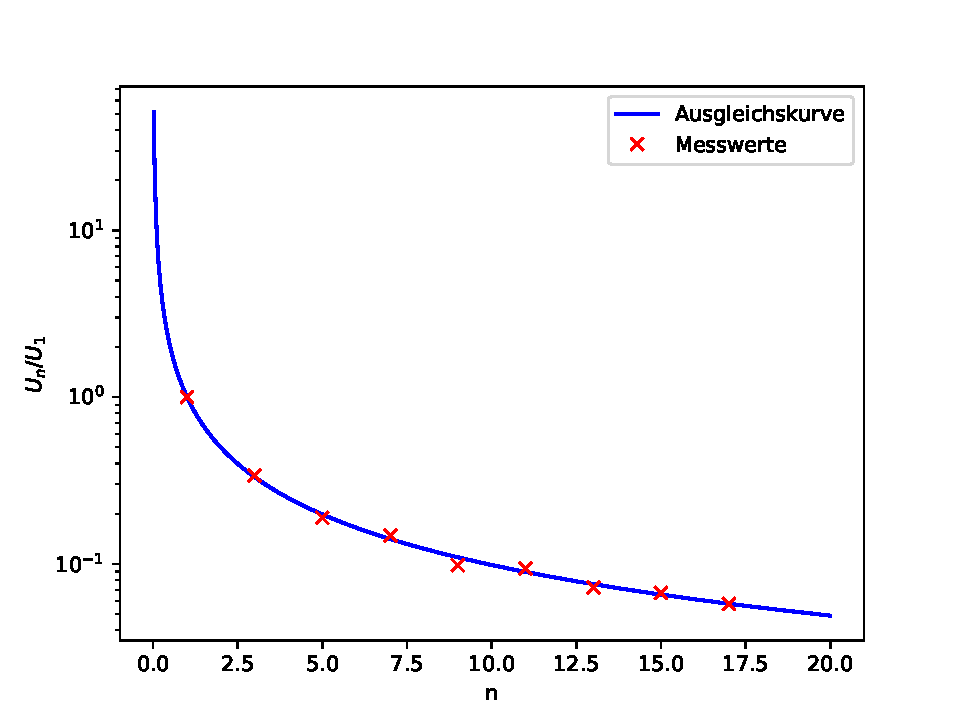
\includegraphics[scale=0,5]{content/images/rechteck.pdf}
\caption{Rechteck-Amplitudenverhältnis in Abhängigkeit von der Zahl der Oberwelle}\label{fig:R}
\end{figure}
Die Regression 
\begin{equation}
\frac{U_.n}{U_.1}(n) = a \cdot n^{-b}\label{eq:Reg}
\end{equation}
liefert für den Koeffizienten:
\[
b_.{Rechteck,mess}= 1,01 \pm 0,01
\]
Der Theorie nach fällt die Kurve einer Rechteck-Spannung mit $\frac{1}{n}$ ab, also gilt:
\[
b_.{Rechteck,theo}= 1
\]
Die Abweichung beträgt somit
\[
\Delta b = 1\% \text{.}
\]
\subsubsection{Sägezahn-Spannung}
Der Funktionen-Generator wird auf eine Frequenz $f=\SI{100e3}{\hertz}$ und eine Spannung von $U_.{Sägezahn} = \SI{1e3}{\volt}$.\newline
Aus den gemessenen Daten wird das Amplitudenverhältnis der $n$-ten Oberwelle zur ersten $\frac{U_.n}{U_.1}$ bestimmt, was in Tabelle \ref{tab:tab2} zu sehen ist.
\begin{table}
	\centering
	\caption{Messdaten der Oberwellen einer Sägezahn-Spannung}
	\sisetup{table-format=1.2}
	\begin{tabular}{S[table-format=3.2] S[table-format=3.2]S[table-format=3.2]S[table-format=3.2]}
		\toprule
		{$n/\si[per-mode=reciprocal]{}$}&{$\nu/10^3/\si[per-mode=reciprocal]{\hertz}$}&{$U_.n/\si[per-mode=reciprocal]{\volt}$}&{$\frac{U_.n}{U_.1}/\si[per-mode=reciprocal]{}$} \\
		\midrule
		1 & 87,5 & 208 & 1 \\
		2 & 187,5 & 96,0 & 0,46 \\
		3 & 287,5 & 72,0 & 0,35 \\
		4 & 387,5 & 54,4 & 0,26 \\
		5 & 487,5 & 40,4 & 0,19 \\
		6 & 587,5 & 34,0 & 0,16 \\
		7 & 681,2 & 32,0 & 0,15 \\
		8 & 781,2 & 26,6 & 0,13 \\
		9 & 875,0 & 21,4 & 0,10 \\
		\bottomrule
	\end{tabular}
	\label{tab:tab2}
\end{table}
\noindent In Abbildung \ref{fig:S} wird das Amplitudenverhältnis gegen die Anzahl der Oberwellen halblogarithmisch aufgetragen.
\begin{figure}
\centering
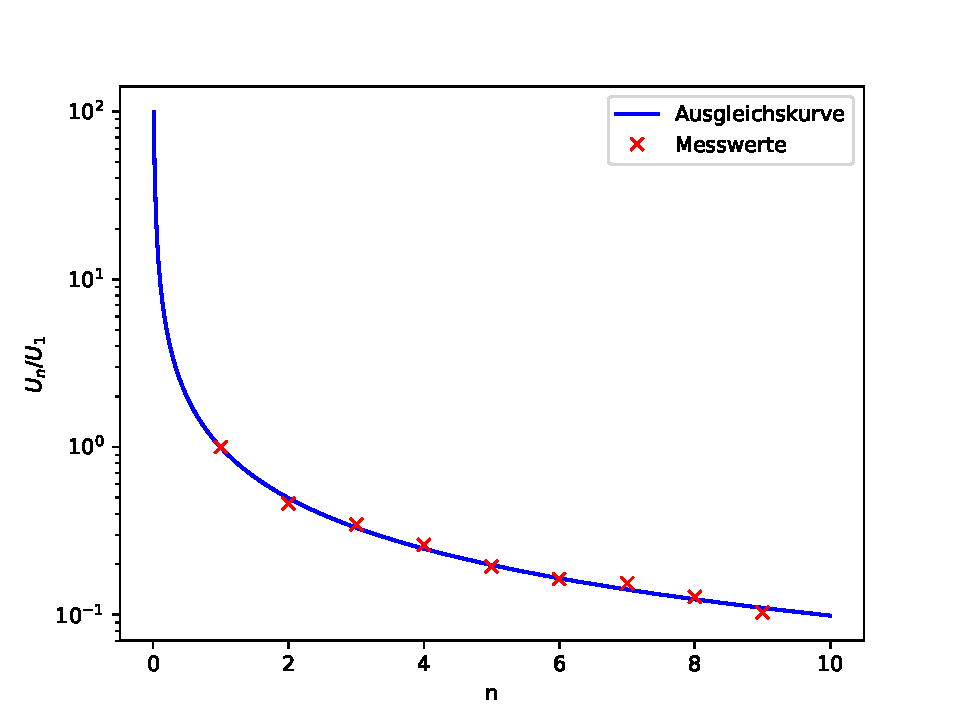
\includegraphics[scale=0,5]{content/images/saegezahn.pdf}
\caption{Sägezahn-Amplitudenverhältnis in Abhängigkeit von der Zahl der Oberwelle}\label{fig:S}
\end{figure}
Die Regression nach Gleichung \eqref{eq:Reg} liefert:
\[
b_.{Sägezahn,mess} = 1,00 \pm 0,02
\]
Dies entspricht dem Theoriewert 
\[
b_.{Sägezahn,theo} = 1
\]


\subsubsection{Dreieck-Spannung}

Der Funktionen-Generator wird auf eine Frequenz $f=\SI{100e3}{\hertz}$ und eine Spannung von $U_.{Dreieck} = \SI{1e3}{\volt}$.\newline
Aus den gemessenen Daten wird das Amplitudenverhältnis der $n$-ten Oberwelle zur ersten $\frac{U_.n}{U_.1}$ bestimmt, was in Tabelle \ref{tab:tab3} zu sehen ist.
\begin{table}
	\centering
	\caption{Messdaten der Oberwellen einer Dreieck-Spannung}
	\sisetup{table-format=1.2}
	\begin{tabular}{S[table-format=3.2] S[table-format=3.2]S[table-format=3.2]S[table-format=3.2]}
		\toprule
		{$n/\si[per-mode=reciprocal]{}$}&{$\nu/10^3/\si[per-mode=reciprocal]{\hertz}$}&{$U_.n/\si[per-mode=reciprocal]{\volt}$}&{$\frac{U_.n}{U_.1}/\si[per-mode=reciprocal]{}$} \\
		\midrule
		1 & 85 & 270 & 1 \\
		3 & 245 & 29,8 & 0,11 \\
		5 & 405 & 11,0 & 0,04 \\
		7 & 565 & 5,0 & 0,02 \\
		9 & 725 & 3,4 & 0,01 \\
		11 & 885 & 2,0 & 0,01 \\
		13 & 1045 & 1,8 & 0,01 \\
		15 & 1205 & 1,3 & 0,004 \\
		\bottomrule
	\end{tabular}
	\label{tab:tab3}
\end{table}
\noindent In Abbildung \ref{fig:D} wird das Amplitudenverhältnis gegen die Anzahl der Oberwellen halblogarithmisch aufgetragen.
\begin{figure}
\centering
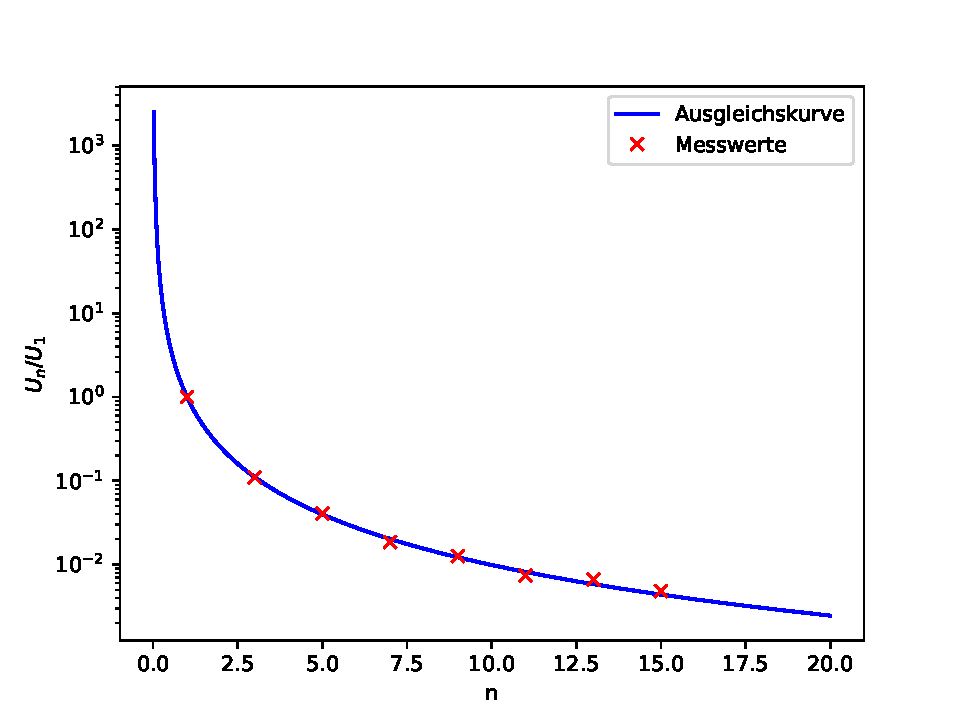
\includegraphics[scale=0,5]{content/images/dreieck.pdf}
\caption{Dreeick-Amplitudenverhältnis in Abhängigkeit von der Zahl der Oberwelle}\label{fig:D}
\end{figure}
Die Regression nach Gleichung \eqref{eq:Reg} liefert:
\[
b_.{Sägezahn,mess} = 2,01 \pm 0,01
\]
Da die Dreieck-Spannung theoretisch mit $\frac{1}{n^2}$ abfällt,  gibt es eine Abweichung zum Theoriewert
\[
b_.{Sägezahn,theo} = 2
\]
von
\[
\Delta b = 0,5\% \text{.}
\]

\subsection{Fourier-Synthese}
Bei allen Synthesen wurden die einzelnen Oberwellen über die Lissajous-Figuren so justiert, dass das bestmögliche Resultat erreicht wurde.
\subsubsection{Rechteck-Spannung}
Eine Rechteck-Spannung von $\SI{100}{\volt}$ wird aus den in Tabelle \ref{tab:tab4} aufgezählten Oberwellen synthetisiert. Das Ergebnis ist in Abbildung \ref{fig:R2} zu sehen.

\begin{table}
	\centering
	\caption{Einstellungen zur Synthese einer Rechteck-Spannung}
	\sisetup{table-format=1.2}
	\begin{tabular}{S[table-format=3.2] S[table-format=3.2]
		\toprule
		{$n/\si[per-mode=reciprocal]{}$}&{$U/\si[per-mode=reciprocal]{\volt}$}\\
		\midrule
		1 & 127 \\
		3 & 42,4 \\
		5 & 25,5 \\
		7 & 18,2 \\
		9 & 14,1 \\
		\bottomrule
	\end{tabular}
	\label{tab:tab4}
\end{table}
\begin{figure}
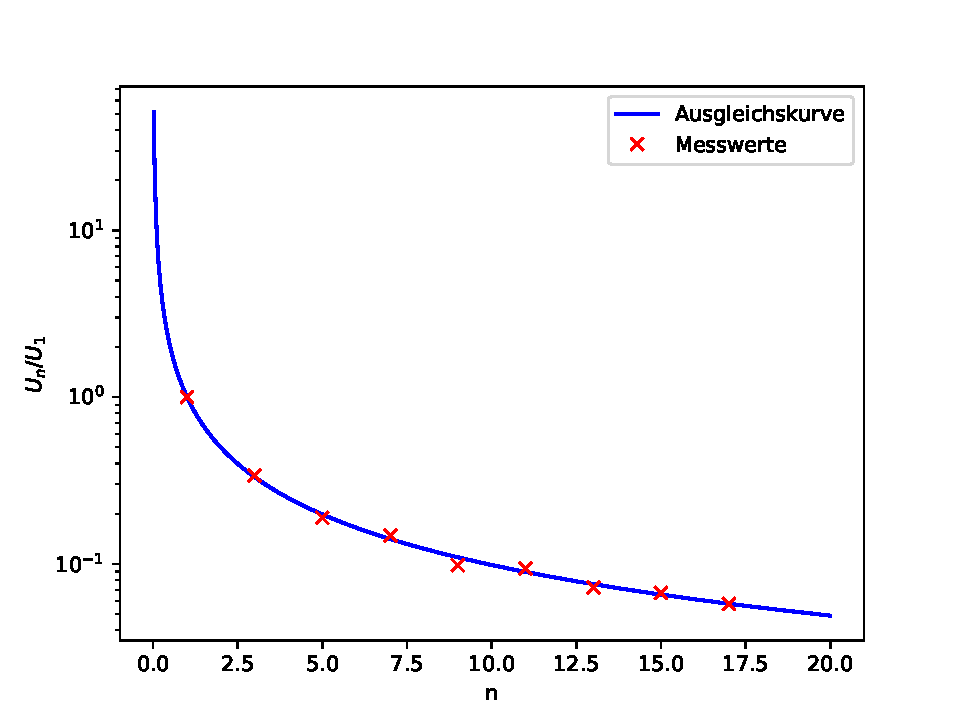
\includegraphics[scale=0.8]{content/images/rechteck.BMP}
\caption{Synthetisierte Rechteck-Spannung}\label{fig:R2}
\end{figure}
\subsubsection{Sägezahn-Spannung}
Eine Sägezahn-Spannung von $\SI{100}{\volt}$ wird aus den in Tabelle \ref{tab:tab5} aufgezählten Oberwellen synthetisiert. Das Ergebnis ist in Abbildung \ref{fig:S2} zu sehen.

\begin{table}
	\centering
	\caption{Einstellungen zur Synthese einer Sägezahn-Spannung}
	\sisetup{table-format=1.2}
	\begin{tabular}{S[table-format=3.2] S[table-format=3.2]
		\toprule
		{$n/\si[per-mode=reciprocal]{}$}&{$U/\si[per-mode=reciprocal]{\volt}$}\\						\midrule
		1 & 63,7 \\
		2 & 31,8 \\
		3 & 21,2 \\
		4 & 15,9 \\
		5 & 12,7 \\
		6 & 10,6 \\
		7 & 9,1 \\
		8 & 8,0 \\
		9 & 7,1 \\
		\bottomrule
	\end{tabular}
	\label{tab:tab5}
\end{table}
\begin{figure}
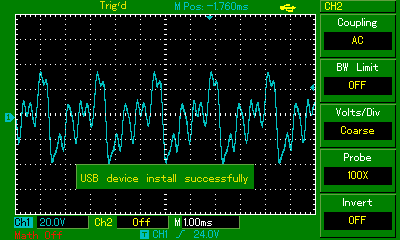
\includegraphics[scale=0.8]{content/images/saegezahn.BMP}
\caption{Synthetisierte Sägezahn-Spannung}\label{fig:S2}
\end{figure}

\subsubsection{Dreieck-Spannung}
Eine Rechteckspannung von $\SI{50}{\volt}$ wird aus den in Tabelle \ref{tab:tab6} aufgezählten Oberwellen synthetisiert. Das Ergebnis ist in Abbildung \ref{fig:D2} zu sehen.

\begin{table}
	\centering
	\caption{Einstellungen zur Synthese einer Dreieck-Spannung}
	\sisetup{table-format=1.2}
	\begin{tabular}{S[table-format=3.2] S[table-format=3.2]
		\toprule
		{$n/\si[per-mode=reciprocal]{}$}&{$U/\si[per-mode=reciprocal]{\volt}$}\\
		\midrule
		1 & 127,3 \\
		3 & 14,1 \\
		5 & 5,1 \\
		7 & 2,6 \\
		\bottomrule
	\end{tabular}
	\label{tab:tab6}
\end{table}
\begin{figure}
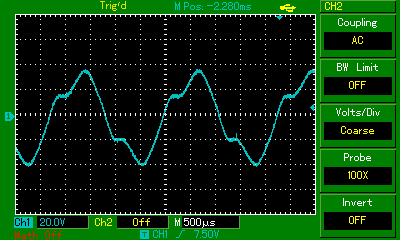
\includegraphics[scale=0.8]{content/images/dreieck.BMP}
\caption{Synthetisierte Dreieck-Spannung}\label{fig:D2}
\end{figure}